\chapter{Instalasi Python}
\section{Sejarah singkat}
Python dibangun oleh Guido van Rossum (\figurename~\ref{fig:guido}\footnote{\url{https://gvanrossum.github.io/images/guido-headshot-2019.jpg}}) pada sekitar tahun 1980 di \textit{Centrum Wiskunde \& Informatica} (CWI) di Belanda\cite{python3intro}. Nama Python diambil dari program TV favorit Guido yang berjudul '''Monty Pythons Flying Circus''' yang tayang pada kisaran tahun 1969-1974.

\begin{figure}
  \begin{center}
    \includegraphics[scale=.5]{pics/guido-headshot-2019.jpg}
    \caption{Guido van Rossum}
    \label{fig:guido}
  \end{center}
\end{figure}

\section{Interpreter Python}
\label{sec:interpreter}
Seperti telah dijelaskan di bagian Pengantar, instalasi \textit{interpreter} Python dilakukan di sistem operasi Windows 7. Tahapan instalasi ini mengasumsikan bahwa tidak ada kendala apapun terkait sistem operasi. Selanjutnya mahasiwa diminta untuk mengunduh \textit{interpreter} Python melalui laman \url{https://www.python.org/downloads/} sesuai kebutuhannya. 

Mengeksekusi unduhan tersebut akan memunculkan dialog seperti pada \figurename~\ref{fig:install1}. Pastikan untuk memilih konfigurasi \texttt{PATH} secara otomatis agar ketika proses instalasi selesai, \textit{interpreter} Python dapat dijalankan dari mana saja di sistem komputer masing-masing. Untuk kondisi di mana terjadi kesalahan, akan muncul dialog yang memberi kita kesempatan untuk melihat \textit{log}. Buka log tersebut dan lihat sumber dari kesalahan instalasi yang sedang terjadi.

\begin{figure}[h!]
   \begin{center}
     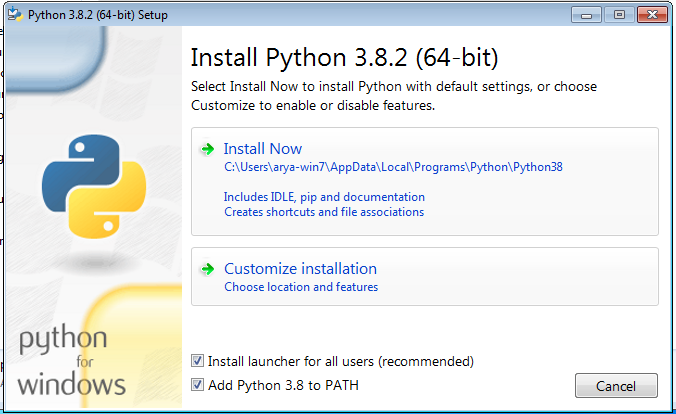
\includegraphics[scale=.5]{pics/installPython1.png}
     \caption{Dialog instalasi \textit{interpreter} Python}
     \label{fig:install1}
   \end{center}
 \end{figure} 

Pilihan opsi \textit{Customize installation} akan menampilkan dialog seperti \figurename~\ref{fig:feature}. Pastikan semua pilihan dipilih. Kemudian, selama proses instalasi berlangsung, pengguna akan disuguhkan dialog seperti \figurename~\ref{fig:installProgres}. Tunggu sampai dialog tanda selesai dikeluarkan seperti pada \figurename~\ref{fig:finish}.

\begin{figure}[h!]
  \begin{center}
    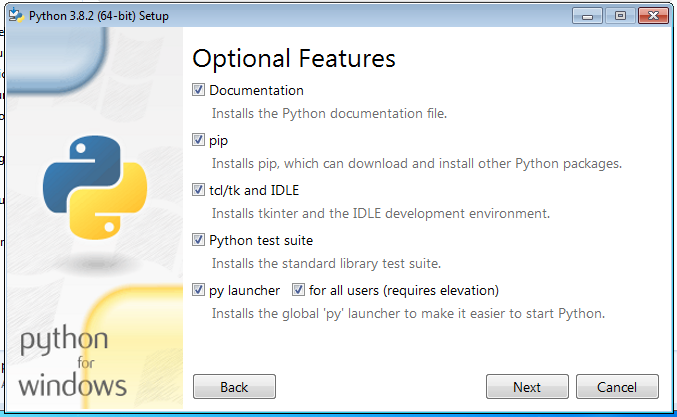
\includegraphics[scale=.5]{pics/featureInstall.png}
    \caption{Pilihan paket pendukung sebelum instalasi dilakukan}
    \label{fig:feature}
  \end{center}
\end{figure}

\begin{figure}[h!]
  \begin{center}
    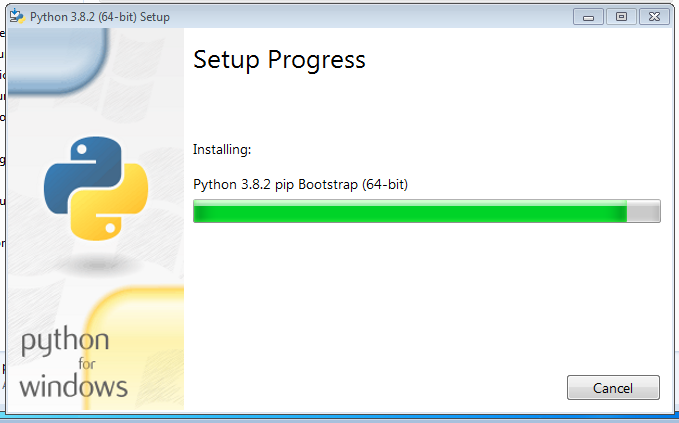
\includegraphics[scale=.5]{pics/installProgress.png}
    \caption{Dialos selama proses instalasi berlangsung}
    \label{fig:installProgres}
  \end{center}
\end{figure}

\begin{figure}[h!]
  \begin{center}
    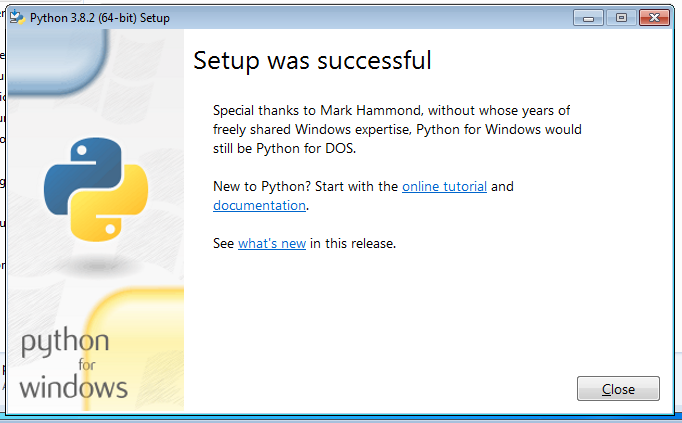
\includegraphics[scale=.5]{pics/installFinished.png}
    \caption{Dialog tanda selesai instalasi}
    \label{fig:finish}
  \end{center}
\end{figure}

Seperti telah ditunjukkan pada \figurename~\ref{fig:install1} tentang informasi lokasi \textit{interpreter} Python diletakkan, dapat juga dibuktikan melalui aplikasi \texttt{CMD} seperti \figurename~\ref{fig:lokasi}. Sedangkan \textit{interpreter} Python dapat diujicobakan dengan menuliskan perintah \texttt{python} di aplikasi \texttt{CMD}. Akan muncul dialog seperti \figurename~\ref{fig:siap}. \textit{Interpreter} Python siap digunakan, ditandai dengan munculnya karakter \texttt{>>>}.

\begin{figure}[h!]
  \begin{center}
    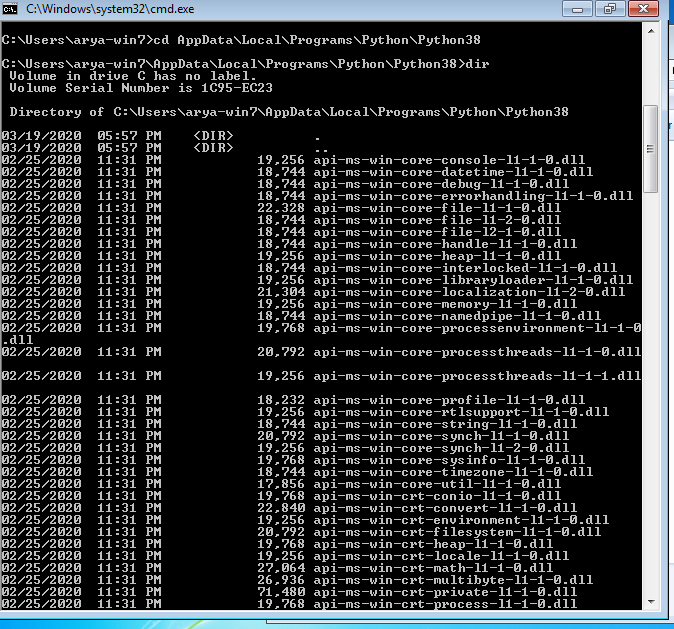
\includegraphics[scale=.5]{pics/installedLocation.png}
    \caption{Lokasi instalasi \textit{interpreter} Python}
    \label{fig:lokasi}
  \end{center}
\end{figure}

\begin{figure}[h!]
  \begin{center}
    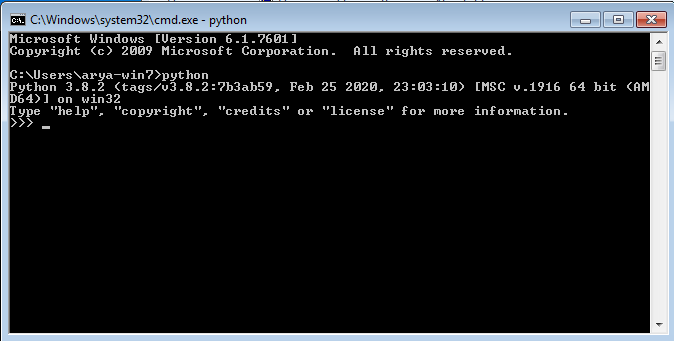
\includegraphics[scale=.5]{pics/pythonAktif.png}
    \caption{\textit{Interpreter} Python siap digunakan}
    \label{fig:siap}
  \end{center}
\end{figure}

Tahapan selanjutnya adalah instalasi pustaka \texttt{scikit-image}. Proses instalasinya dilakukan dengan aplikasi pengelola paket Python yang bernama \texttt{pip}. Silakan lihat \figurename~\ref{fig:feature}. \texttt{pip} ada di urutan kedua dari fitur tambahan. \texttt{pip} dapat digunakan untuk melihat paket apa saja yang telah terpasang di sistem kita. Caranya dengan menjalankan perintah \texttt{python -m pip list} seperti ditunjukkan \figurename~\ref{fig:daftarPaket}.

\begin{figure}[h!]
  \begin{center}
    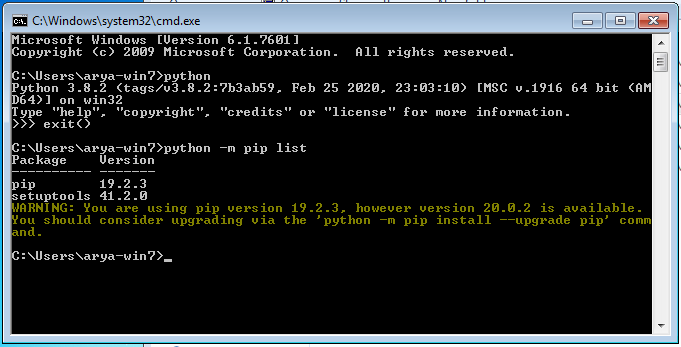
\includegraphics[scale=.5]{pics/pipList.png}
    \caption{Daftar paket yang terpasang}
    \label{fig:daftarPaket}
  \end{center}
\end{figure}

\texttt{pip} dapat juga digunakan untuk meng-\texttt{upgrade} paket yang telah terpasang, bahkan dirinya sendiri. Untuk meng-\textit{upgrade} paket \texttt{pip} itu sendiri, dapat dilakukan dengan menjalankan perintah \texttt{python -m pip install --upgrade pip} seperti \figurename~\ref{fig:pipUpgrade}. Perhatikan versi \texttt{pip} yang ada di \figurename~\ref{fig:daftarPaket} dan \figurename~\ref{fig:pipUpgrade}.
 
\begin{figure}
  \begin{center}
    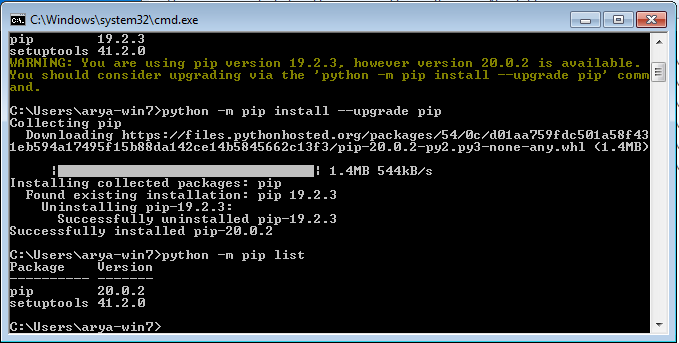
\includegraphics[scale=.5]{pics/pipList2.png}
    \caption{Hasil \texttt{upgrade} pip}
    \label{fig:pipUpgrade}
  \end{center}
\end{figure}

Sedangkan untuk memasang pustaka \texttt{scikit-image}, jalankan perintah \texttt{python -m pip install scikit-image} pada aplikasi \texttt{CMD} seperti \figurename~\ref{fig:installSkimage}.

\begin{figure}[h!]
  \begin{center}
    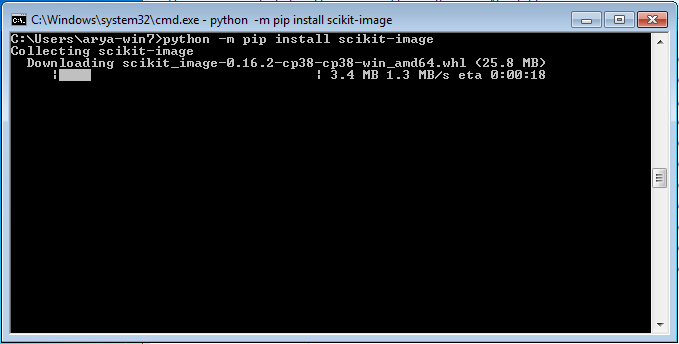
\includegraphics[scale=.5]{pics/installScikit-Image.png}
    \caption{Instalasi pustaka \texttt{scikit-image} menggunakan \texttt{pip}}
    \label{fig:installSkimage}
  \end{center}
\end{figure}

Jika ada pustaka lain yang menjadi ketergantungan dari pustaka yang akan diinstal, pip akan melakukan instalasi secara otomatis. \figurename~\ref{fig:installDepend} menunjukkan proses tersebut. Hal ini akan sangat memudahkan pengguna mengelola pustaka Python yang digunakan.

\begin{figure}[h!]
  \begin{center}
    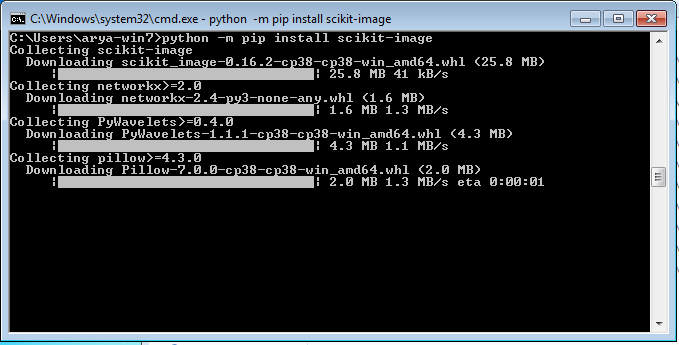
\includegraphics[scale=.5]{pics/installScikit-Imagedependencies.png}
    \caption{Instalasi pustaka \textit{dependent}}
    \label{fig:installDepend}
  \end{center}
\end{figure}

Setelah selesai, kita dapat kembali melihat daftar paket yang terpasang melalui pengelolaan \texttt{pip} yang ditunjukkan \figurename~\ref{fig:daftarPaket2}.

\begin{figure}[h!]
  \begin{center}
    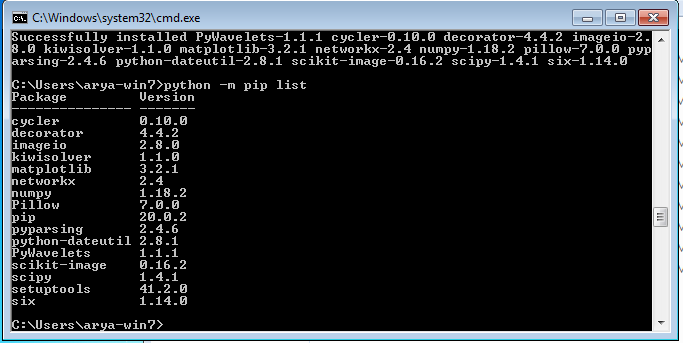
\includegraphics[scale=.5]{pics/pipList3.png}
    \caption{Daftar terakhir paket terpasang}
    \label{fig:daftarPaket2}
  \end{center}
\end{figure}

Menu aplikasi pendukung Python akan muncul seperti \figurename~\ref{fig:menu}. Menu kedua pada \figurename~\ref{fig:menu} akan memunculkan aplikasi \texttt{CMD} yang sama dengan yang ditunjukkan \figurename~\ref{fig:siap}, tetapi tanpa perlu memanggil perintah \texttt{python} terlebih dahulu. CMD secara otomatis akan memunculkan Python \texttt{shell} seperti \figurename~\ref{fig:siap}.

\begin{figure}[h!]
  \begin{center}
    \includegraphics[scale=.5]{pics/menuPython.png}
    \caption{Daftar menu aplikasi pendukung Python}
    \label{fig:menu}
  \end{center}
\end{figure}

\texttt{IDLE} adalah antarmukan \textit{interpreter} Python seperti ditunjukkan \figurename~\ref{fig:idle}. Dalam \figurename~\ref{fig:idle} juga terlihat bahwa kita berhasil meng-\textit{import} pustaka \texttt{scikit-image}, yang dalam \texttt{IDLE} di Windows 7 disebut sebagai \texttt{skimage}. Jika Anda sedang menggunakan Ubuntu, kemudian menggunakan pustaka \texttt{scikit-image} yang diperoleh dari \textit{repository} Ubuntu (bukan dari \texttt{pip}), pustaka \texttt{scikit-image} juga di-\textit{import} dengan nama \texttt{skimage}. Berhasilnya sebuah pustaka Python di-\textit{import} adalah ketika tidak ada komentar yang muncul setelah perintah \texttt{import} tersebut.

\begin{figure}
  \begin{center}
    \includegraphics[scale=.5]{pics/idle.png}
    \caption{Aplikasi \texttt{IDLE}}
    \label{fig:idle}
  \end{center}
\end{figure}

Selanjutnya, jika ditemukan petunjuk untuk masuk ke Python \texttt{Shell}, Anda dapat menggunakan aplikasi \texttt{IDLE}\texttt{}, atau menggunakan terminal (di Linux)/\texttt{CMD} (di Windows) dengan terlebih dahulu menjalankan perintah \texttt{python}.

\section{Anaconda}
Selain pilihan manual seperti yang telah dijelaskan di Sub bab \ref{sec:interpreter}, Anaconda bisa menjadi opsi lain yang lebih bersifat otomatis. Saya menyebutnya otomatis karena Anaconda sejumlah pustaka Python, terutama yang banyak digunakan di \textit{Data Mining}, \textit{Machine Learning} atau \textit{Data Science} telah dikemas di dalam Anaconda. Bahkan beberapa editor yang populer untuk Python juga dikemasnya. Anaconda bahkan mengemasnya khusus untuk \textit{platform} yang berbeda. Anda dapat menghubungi alamat \url{https://www.anaconda.com/} untuk mengunduh aplikasinya. Sesuaikan kebutuhan Anda dengan pilihan yang ada seperti ditunjukkan \figurename~\ref{fig:platformAnaconda}.

\begin{figure}[h!]
  \begin{center}
    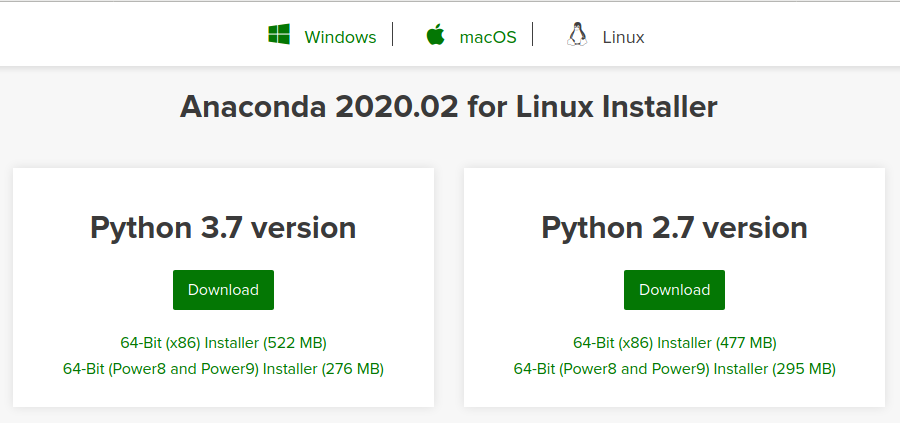
\includegraphics[scale=.5]{pics/anacondaInstall0.png}
    \caption{Pilihan \textit{platform} instalasi Anaconda}
    \label{fig:platformAnaconda}
  \end{center}
\end{figure}

Instalasi Anaconda akan menghadirkan dialog seperti ditunjukkan \figurename~\ref{fig:pembuka} - \figurename~\ref{fig:instalasiEnd}. Anaconda akan meletakkan pustaka di lokasi \texttt{C:\textbackslash\textbackslash ProgramData\textbackslash\textbackslash Anaconda3} yang berbeda dengan \texttt{pip} seperti terlihat di \figurename~\ref{fig:target}. Sedangkan di \figurename~\ref{fig:prosesInstalasi} terlihat sejumlah pustaka penting seperti \texttt{scikit-image} dan \texttt{scikit-learn} tengah diinstal. 

\begin{figure}aplikasi ini akan menghadirkan antarmuka seperti tampak
  \begin{center}
    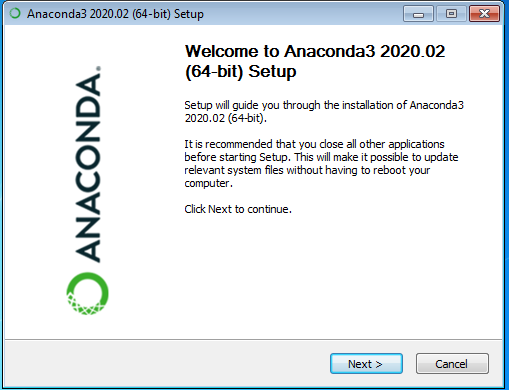
\includegraphics[scale=.5]{pics/anacondaInstall1.png}
    \caption{Dialog pembuka instalasi}
    \label{fig:pembuka}
  \end{center}
\end{figure}

\begin{figure}[h!]
  \begin{center}
    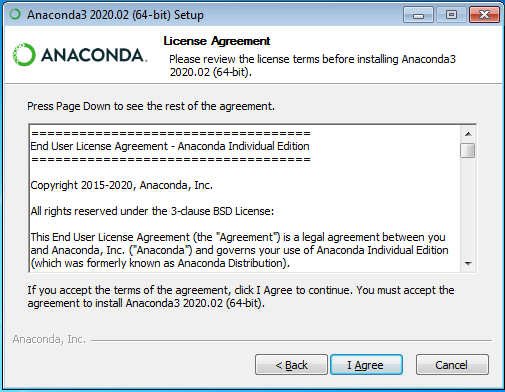
\includegraphics[scale=.5]{pics/anacondaInstall2.png}
    \caption{Menyetujui kesepakatan}
    \label{fig:kesepakatan}
  \end{center}
\end{figure}

\begin{figure}[h!]
  \begin{center}
    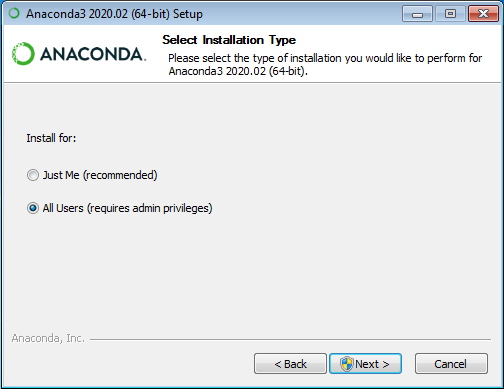
\includegraphics[scale=.5]{pics/anacondaInstall3.png}
    \caption{Pilihan pengguna Anaconda}
    \label{fig:pengguna}
  \end{center}
\end{figure}

\begin{figure}[h!]
  \begin{center}
    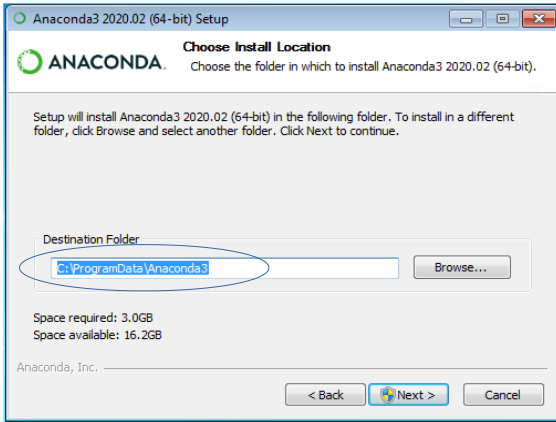
\includegraphics[scale=.5]{pics/anacondaInstall4a.png}
    \caption{Target instalasi}
    \label{fig:target}
  \end{center}
\end{figure}

\begin{figure}[h!]
  \begin{center}
    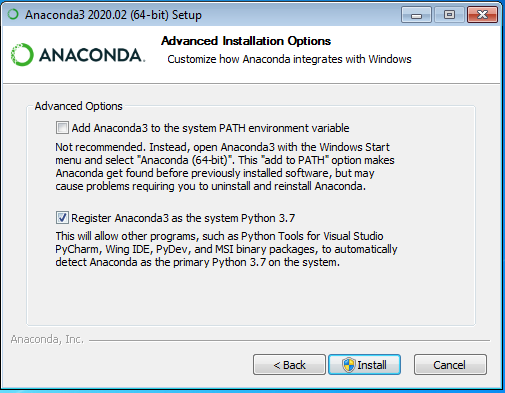
\includegraphics[scale=.5]{pics/anacondaInstall5.png}
    \caption{Menjadikan Anaconda sebagai sistem utama Python}
    \label{fig:utama}
  \end{center}
\end{figure}

\begin{figure}[h!]
  \begin{center}
    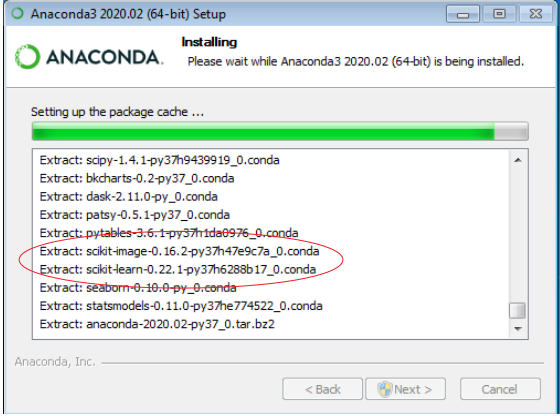
\includegraphics[scale=.5]{pics/anacondaInstall6a.png}
    \caption{Proses instalasi}
    \label{fig:prosesInstalasi}
  \end{center}
\end{figure}

\begin{figure}[h!]
  \begin{center}
    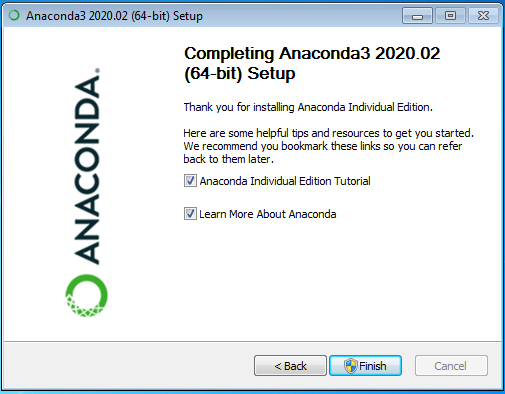
\includegraphics[scale=.5]{pics/anacondaInstall9.png}
    \caption{Instalasi selesai}
    \label{fig:instalasiEnd}
  \end{center}
\end{figure}

Instalasi Anaconda akan membuat menu seperti pada \figurename~\ref{fig:menuAnaconda}. Di situ terlihat sejumlah aplikasi yang dapat digunakan untuk mengembangkan kode komputer berbasis Python seperti Jupyter dan Spyder. Untuk Jupyter, aplikasi ini akan menghadirkan antarmuka seperti tampak pada \figurename~\ref{fig:jupyter}. Di sisi kanan atas terlihat beberapa opsi antarmuka untuk mengelola proyek Python dengan Jupyter, seperti Terminal \figurename~\ref{fig:jupyterTerminal} atau Python \texttt{Shell} di bawah Jupyter seperti \figurename~\ref{fig:jupyterShell} yang perannya seperti \texttt{IDLE} di \figurename~\ref{fig:idle}. Sedangkan untuk Spyder, akan tampak antarmuka seperti \figurename~\ref{fig:spyder}.

\begin{figure}[h!]
  \begin{center}
    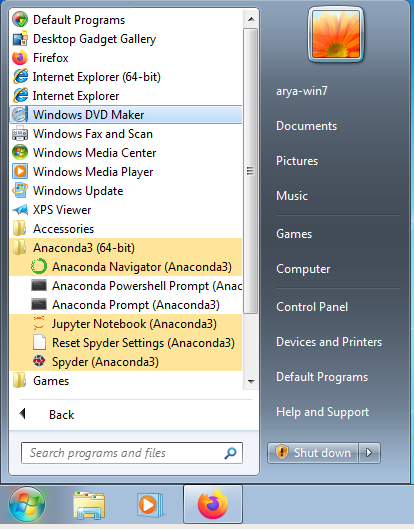
\includegraphics[scale=.5]{pics/anacondaMenu2.png}
    \caption{}
    \label{fig:menuAnaconda}
  \end{center}
\end{figure}

\begin{figure}
  \begin{center}
    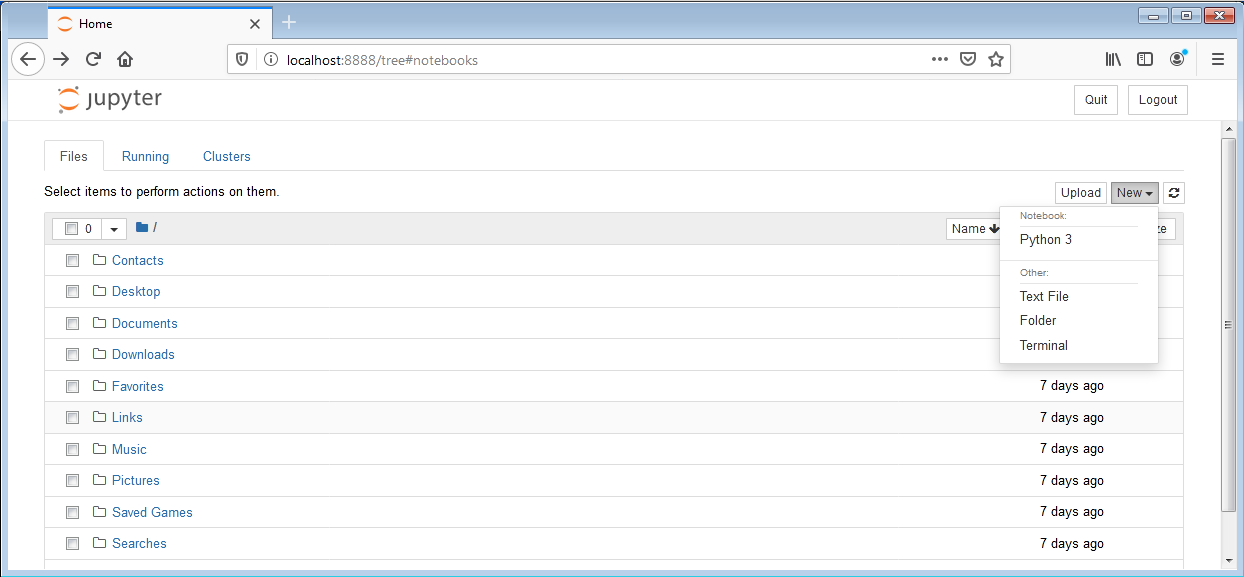
\includegraphics[scale=.5]{pics/jupyter2.png}
    \caption{Aplikasi \texttt{Jupyter}}
    \label{fig:jupyter}
  \end{center}
\end{figure}

\begin{figure}
  \begin{center}
    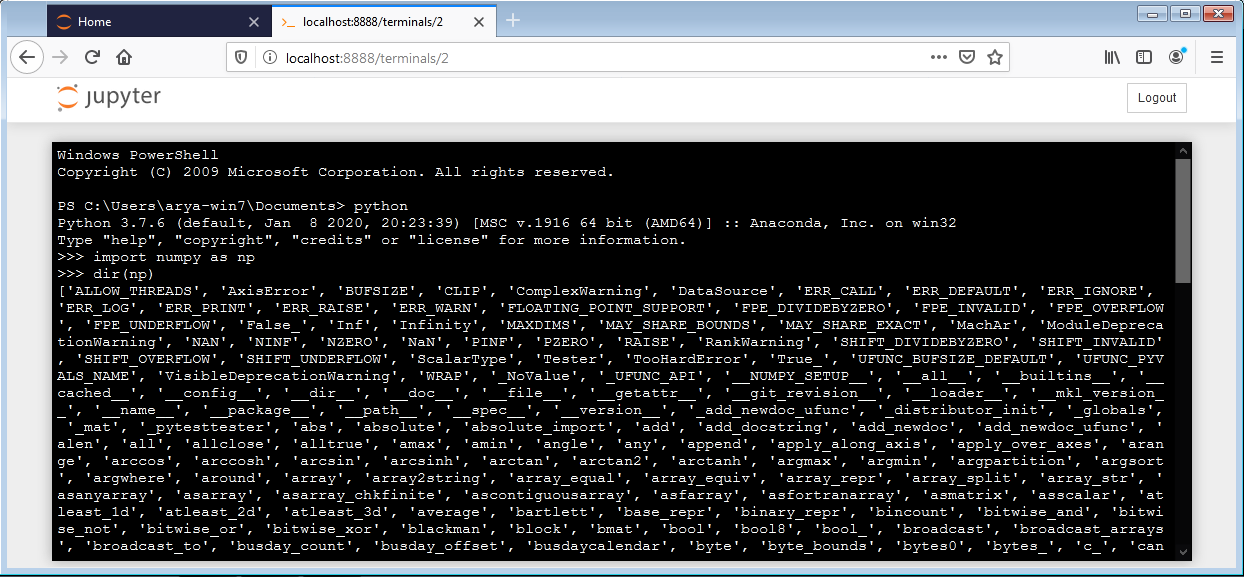
\includegraphics[scale=.5]{pics/jupyter3.png}
    \caption{Terminal pada aplikasi \texttt{Jupyter}}
    \label{fig:jupyterTerminal}
  \end{center}
\end{figure}

\begin{figure}
  \begin{center}
    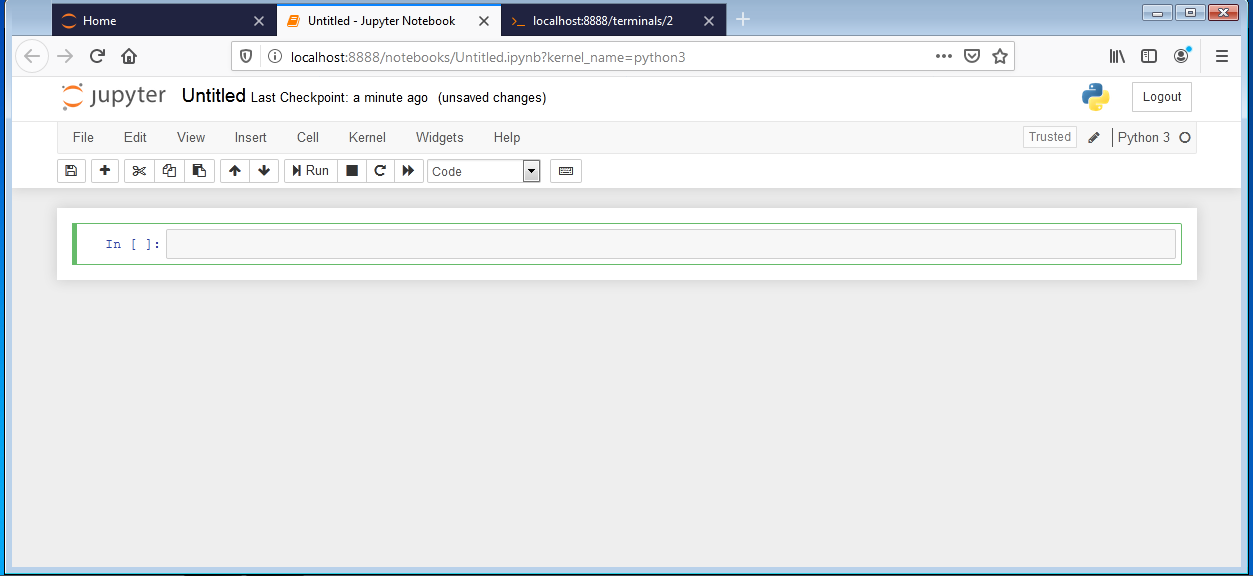
\includegraphics[scale=.5]{pics/jupyter4.png}
    \caption{Python \texttt{Shell} pada aplikasi \texttt{Jupyter}}
    \label{fig:jupyterShell}
  \end{center}
\end{figure}

\begin{figure}[h!]
  \begin{center}
    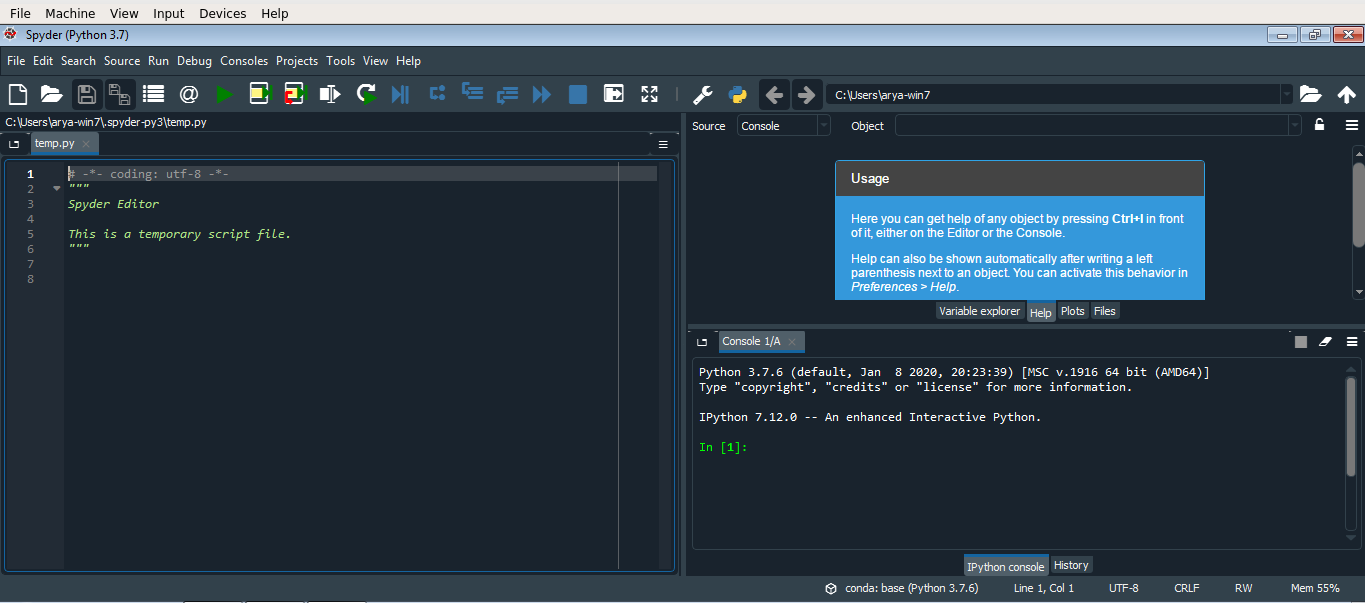
\includegraphics[scale=.45]{pics/spyder.png}
    \caption{Aplikasi \texttt{Spyder}}
    \label{fig:spyder}
  \end{center}
\end{figure}
